\documentclass[11pt, letterpaper, twoside]{article}
\usepackage[letterpaper, portrait, left=1in, right=1in, top=1in, bottom=1in]{geometry}\usepackage{amsmath}
\usepackage{amssymb}
\usepackage{graphicx}
\usepackage[explicit]{titlesec}
\usepackage{epstopdf}
\usepackage{amsmath}
\usepackage{inputenc}
\usepackage{enumitem}
\usepackage{booktabs, multirow} %for borders and merged ranges
\usepackage{soul}% for underlines
\usepackage[table]{xcolor} % for cell colors
\newcommand\aug{\fboxsep=-\fboxrule\!\!\!\fbox{\strut}\!\!\!} %Use \aug to make a equal column for an augmented matrix. Ie. 1 & 2 & 3 & 4 & \aug & x \\
\begin{document}
\begin{titlepage}
\centering
\vspace*{60px}
\hspace{0pt}

\includegraphics[width=0.2\textwidth]{logo}\par\vspace{1cm}
{\scshape\LARGE Athabasca University \par}
\vspace{1cm}
{\scshape\Large MATH 265\par}
\vspace{1.5cm}
{\huge\bfseries Assignment 4\par}
\vspace{2cm}
{\Large\itshape Stanley Zheng\par}
\vfill
{\large October 17, 2020\par}
\vspace*{50px}
\hspace{0pt}
\pagebreak
\end{titlepage}

\noindent My sincere apologies if there are any typos or work is not shown fully. 
I wrote this assignment hastily, and the length made it difficult to check for typos. 
I hope you can understand. Thanks.
\begin{enumerate}
\item 
\begin{enumerate}[label=\alph*)]
\item ‌‌ 

\vspace{0.2cm}
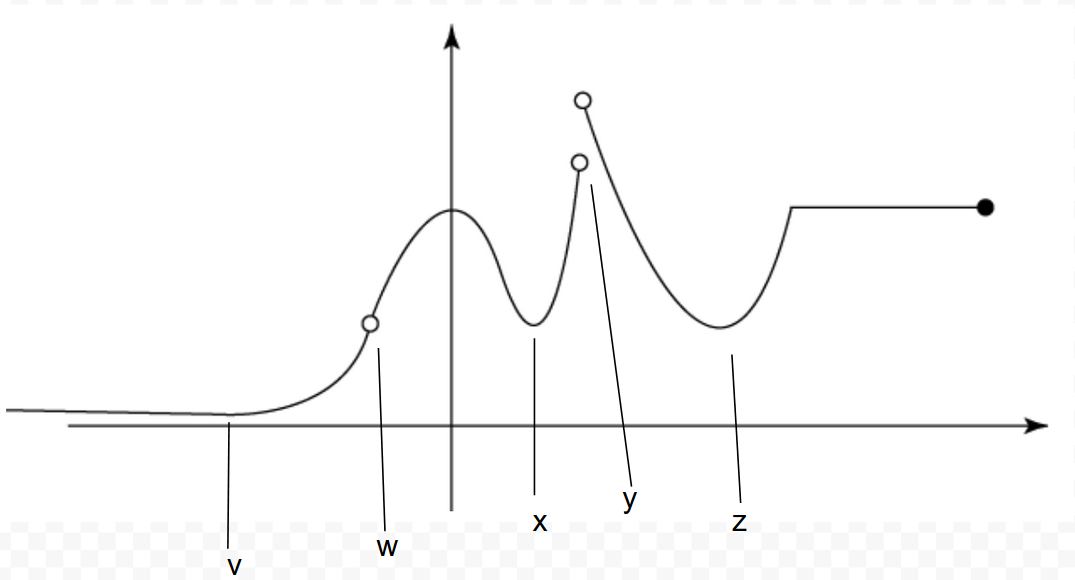
\includegraphics[width=0.7\textwidth]{q1}\par

The domain of the function \(g\) is \((-\infty, w)\cup(w, x)\cup(x, y]\)
\item The function \(g\) is continuous from \((-\infty, w)\cup(w, x)\cup(x, y]\).
\item The local maximum ix at \(x=0\), since the derivative is 0.
\item The local minimum is at two points, \(x\) and \(z\), where the derivative is zero.
\item There is no absolute maximum as the derivative at \(y\) is undefined, and \(y\) is not included in the domain.
\item The absolute minimum is at \(v\). It appears as though the graph has negative slope as \(x\) decreases beyond \(v\) to infinity.
\end{enumerate}
\item %q2
The first condition specifies that this is an odd function, so we must verify this by reflecting over the origin.

\item %q3
Our first step is to find the domain of the function.
Setting the denominator to zero, we have \(x^2+6=0\), so our domain is \(x\neq\pm\sqrt6\)

Next, we can find the intercepts. We can find the \(x\) intercept by letting \(y=0\).
We have \(x^2=4\), so our \(x\)-intercepts are \(x=\pm2\).
Likewise, our \(y\)-intercepts are \(-\frac{4}{6}\).

We can then test if the function is even or odd. 
We can test whether it is even or not by simplifying \(f(-x)\). 
If \(f(-x)=f(x)\), then our function is even.
\[f(-x)=\frac{(-x)^2-4}{(-x)^2+6}\]
Since \(-x\) is squared, we know that \(f(-x)=f(x)\), and therefore, the function is even.

Our function is not periodic, but it does have a horizontal asymptote. 
At extremely large values of \(x\), our function will be approximately equal to \(\frac{x^2}{x^2}\), so we have a horizontal asymptote at \(x=1\).

Next, we find the derivative of \(f(x)\).
\[f^\prime(x)=\frac{2x(x^2+6)-2x(x^2-4)}{(x^2+6)^2}\]
\[f^\prime(x)=\frac{20x}{(x^2+6)^2}\]
Since \(f^\prime(x)<0\) when \(x<0\) and \(f^\prime(x)>0\) when \(x>0\), we know that the function is decreasing on \((-\infty, 0)\) and increasing on \(0, \infty\).

Our only critical number is \(x=0\), where \(f^\prime\) changes from positive to negative.
We know it is a local minimum since the derivative to the right is positive, but negative to the left.

We can find concavity with the second derivative of the function. 
\[f^{\prime\prime}(x)=-\frac{60x^2-120}{(x^2+6)^3}\]
From this, the curve is concave upward at \((-\sqrt2, \sqrt2)\) and points of concavity are \(\pm\sqrt2\).

Finally, we can draw the graph of the function.

%GRAPH

\item %q4 (no check)
First, we need to find relative distances for swimming and jogging.
Let's let \(\angle PWE\) be \(\theta\).
We can create a triangle by connecting points \(PWE\) with straight lines.
We know from Thale's theorem that an angle inscribed across the diameter of a circle is always \(90^\circ\), so this triangle is a right triangle.
Then, the swimming distance, line \(PW\), is \(3\cos\theta\).
The arc length for jogging is \(\theta r\), and our diameter is 3km, so the jogging distance is \(2\cdot1.5\theta\). 
We must multiply by 2 since the angle is not measured at the center of the circle, but rather subtends it.

We know that critical points are found where the derivative of a function is 0 or undefined.
To find the derivative, we can find an equation for the time of the journey, then differentiate.
\[\frac{1}{24}\cdot3\theta+\frac{1}{3}\cdot3\cos\theta\]
\[\frac{\theta}{8}+\cos\theta\]
We can then differentiate and find zeros.
\[0=\frac{1}{8}-\sin\theta\]
\[\sin\theta=\frac{1}{8}\]
\[\sin^{-1}\left(\frac{1}{8}\right)=\theta\]
We have \(\theta\approx0.125\). 
To find the distance to jog, we multiply by 3.
The final distance Peter should jog to arrive at point W in the least amount of time is \(\boxed{0.376\text{km}}\)

\item %q5
\begin{enumerate}[label=\alph*)]
\item Graph is as follows:

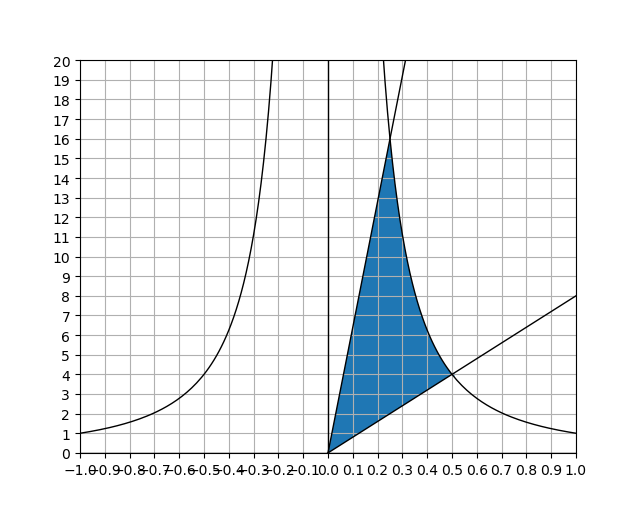
\includegraphics[width=0.6\textwidth]{q5}\par\vspace{1cm}
\item We can evaluate the function at various reference angles, since we know that \(x^2\) will always be positive and \(\sin x\) has a maximum value of 1.

When \(x=0\), we have \(\sin0-(0^2)=0\).

When \(x=\frac{\pi}{2}\), we have \(\sin\frac{\pi}{2}-(\frac{\pi}{2})^2\), which is positive.

When \(x=\frac{\pi}{3}\), we have \(\sin\frac{\pi}{3}-(\frac{\pi}{3})^2\), which is negative.

When \(x=\frac{\pi}{4}\), we have \(\sin\frac{\pi}{4}-(\frac{\pi}{4})^2\), which is positive.

Then, we know that the interval in which \(x\) is nonzero is \([\frac{\pi}{4}, \frac{\pi}{3}]\)

\item 
In order to use Newton's method, we must have the function in the form \(f(x)=0\), so our function is \(\sin x - x^2=0\).

We can now write down the general formula for Newton's method.
\[x_{n+1}=x_n-\frac{\sin x_n-x_n^2}{\cos x_n -2x_n}\]
Next, we can get our first approximation by substituting our lower bound, \(\frac{\pi}{3}\).
\[x_1=\frac{\pi}{3}-\frac{\sin(\frac{\pi}{3})-\left(\frac{\pi}{3}\right)^2}{\cos(\frac{\pi}{3})-2\left(\frac{\pi}{3}\right)}\approx0.902567586\]
We must do this again, but substituting \(x_n\) with 0.902567586.
\[x_2=0.902567586-\frac{\sin0.902567586-\left(0.902567586\right)^2}{\cos0.902567586-2\left(0.902567586\right)}\approx0.8775090289\]
Again, we can substitute \(x_n\) with 0.8775090289.
\[x_3=0.8775090289-\frac{\sin0.8775090289-\left(0.8775090289\right)^2}{\cos0.8775090289-2\left(0.8775090289\right)}\approx0.8767269756\]

After one more repetition, we get \(x_4=0.876726215396\), which has 6 digits consistent with \(x_3\).
Therefore, \(x\) has a nonzero solution of \(\boxed{x=0.876726}\)

\end{enumerate}

\item %q6
We can begin by finding the integral of the first function to see if the ant walks 4cm in the first second.
\[\int_0^1(5t)dt=\frac{5t^2}{2}=\frac{5}{2}\]
The ant can only walk 2.5cm in the first second, therefore, we need to find the integral of the second function.
\[\int_1^t(6\sqrt t-\frac{1}{t})dt=4t^{\frac{3}{2}}-\ln t\]
We can then add our first integral to the second integral and equate it to 4cm.
\[4=\frac{5}{2}+4t^{\frac{3}{2}}-\ln t \]
We have \(t\approx0.266\) for our second function. 
Adding 1 second from our first function, the ant travelled for \(\boxed{1.266s}\).

\item %q7
\begin{enumerate}[label=\alph*)]
\item We can use \(u\) substitution. 
First, we substitute \(u=x^2-6x+1\), the polynomial under the square root.
\[u^\prime=2x-6 dx\]
\[\frac{u^\prime}{2}=x-3dx\]
Conveniently, we see that the numerator has a factor of this.

\begin{align*}
&3\int \frac{\frac{u^\prime}{2}}{\sqrt{u}}\\
&= 3u^{0.5}+c\\
&= \boxed{3\sqrt(x^2-6x+1)+C}
\end{align*}
\item Again, we can use \(u\) substitution, this time, 
we can substitute \(u=3-\tan\theta\), the numerator of the integral.

The derivative is 
\[u^\prime=-\sec^2\theta d\theta\]
Simplifying to find \(\cos^2\theta\), we have \(-u^\prime=\frac{d\theta}{cos^2\theta}\)

Our integral becomes \(\int u (-du)\). 

Again, we can simplify, and our final answer is \(\boxed{\frac{-(3-\tan\theta)^2}{2}+C}\)

\item We can begin by expanding the numerator.
\begin{align*}
&\int\frac{(2-x+x^2)^2}{\sqrt x}\\
&=\int\frac{x^4-2x^3+5x^2-4x+4}{\sqrt x}\\
&=\int x^{\frac{7}{2}}-2x^{\frac{5}{2}}+5x^{\frac{3}{2}}-4x^{\frac{1}{2}}+4x^{-\frac{1}{2}}
\end{align*}
From here, we can simply find the anti-derivative with the equation \(\int x^ndx=\frac{x^{n+1}}{n+1}+C\).
\[\boxed{\frac{2x^{\frac{9}{2}}}{9}-\frac{4x^{\frac{7}{2}}}{7}+2x^{\frac{5}{2}}-\frac{8x^{\frac{3}{2}}}{3}+8\sqrt x+c}\]

\item We can begin by using trigonometric identities to simplify the integral.
\[\int\frac{1+\cos(6x)}{2}dx\]
Then, we can remove the constant and apply the sum rule
\[\frac{1}{2}\int 1dx + \int \cos(6x)dx\]
Finally, evaluating the integrals, we have 
\[\boxed{\frac{x}{2}+\frac{\sin(6x)}{12}+C}\]
\end{enumerate}
\item %q8
%def taken from http://www.sosmath.com/calculus/diff/der11/der11.html
Mean value theorem states that \(f(x)\) is defined and continuous on the interval \([a, b]\) and is differentiable on interval \((a,b)\),
then there is at least one number \(c\) such that \(f^\prime(c)=\frac{f(b)-f(a)}{b-a}\).

For this question, we can let \(f(x)=\cos(x)\). 
Plugging into our equation, we have 
\[f^\prime(c)=\frac{\cos(a)-\cos(b)}{b-a}\]
We can put absolute value to the left-hand side as well as the denominator and numerator.
\[|f^\prime(c)|-\frac{|\cos(a)-\cos(b)|}{|b-a|}\]
We know that \(f(c)=\cos(c)\), so \(f^\prime(c)=-\sin(c)\), and the domain is \([-1, 1]\).
Therefore, we have 
\[|a-b|\geq |cos\prime(c)||a-b|\]
This is since the largest possible value of of \(\cos^\prime(c)\) and \(|a-b|\) is 1.

\item %q9 
\begin{enumerate}[label=\alph*)]
\item
We can use the intermediate value theorem to find possible intervals of a root. 
To this, we can evaluate the function at a few points. 
Looking at the equation, it is not defined when \(x<0\). 
We can start with points \(x=0, 1, 2\).

When \(x=0\): \(f(0)=3\cdot0^3+\sqrt{0}-2=-2\)

When \(x=0.25\): \(f(0.25)=3\cdot0^3+\sqrt{0.25}-2=-1.3125\)

When \(x=1\): \(f(1)=3\cdot1^3+\sqrt(1)-2=2\)

\item
We can use Rolle's theorem and argue by contradiction.
It states that for a function with two real roots, \(a\) and \(b\), we would have \(f(a)=f(b)=0\).

Since \(f\) is a polynomial, it must be differentiable on \((a, b)\) and continuous on \([a,b]\).

Then, we need to find a number \(c\) between \(a\) and \(b\) such that \(f^\prime(c)=0\).

The derivative of our equation is \(9x^2+\frac{1}{2\sqrt x}\)

Given our bound \((0.25, 1)\), this is impossible since \(9x^2\geq0\) and \(x>0.25\) so also \(\frac{1}{2\sqrt x}>0\).

Thus, we have a contradiction and our function \(f\) has exactly one root.

\end{enumerate}
\item %q10
We can first split the integral into parts to use the trigonometric identity.
\[\int \cos^2(x)\cos(x)\sin^2(x)dx\]
Next, we will substitute \(\cos^2(x)=1-\sin^2(x)\)
\[\int(1-\sin^2(x))\cos(x)\sin^2(x)dx\]
We can then use \(u\) substitution, with \(u=\sin(x)\). 
\[\int u^2(1-u^2)du\]
\[\int u^2du = \frac{u^3}{3}\]
\[\frac{u^3}{3}-\frac{u^5}{5}\]
Therefore, after substituting \(u=\sin(x)\) back in, our solution is 
\[\frac{sin^3(x)}{3}-\frac{sin^5(x)}{x}+C\]

\item %Q11
\begin{enumerate}[label=\alph*)]
\item  %q11a
\end{enumerate}

\item %Q12
Let \(a\) be a constant in the interval \((-x, x^2)\).

From the fundamental theorem of calculus, we can split the integral into two parts. 
First, we have 
\[\frac{d}{dx}\int_x^a f(t)dt+\int_a^{x^2}f(t)dt\]
\[=\frac{d}{dx}-\int_{-a}^{-x}f(t)dt\int_a^{x^2}f(t)dt\]
Let \(g(x)\) be the anti-derivative of \(\tan(3x)\). Then, \(g^\prime(x)=\tan(3x)\).

Then, we can rewrite the integral above as the following.
\[\frac{d}{dx}g(x^2)-g(-x)\]
We can then differentiate this using the chain rule
\[2x\cdot g^\prime(x^2)+g^\prime (-x)\]
Recalling \(g^\prime=\tan (x) = f(x)\)

We have \(2x\cdot f(x^2)+f(-x)\). 
Substituting \(f(x)=\tan(3x)\), we have \(\boxed{2x\cdot\tan(3x^2)+\tan(-3x)}\)

\item %Q13


\item %Q14
\begin{enumerate}[label=\alph*)]
\item The graph is as follows:

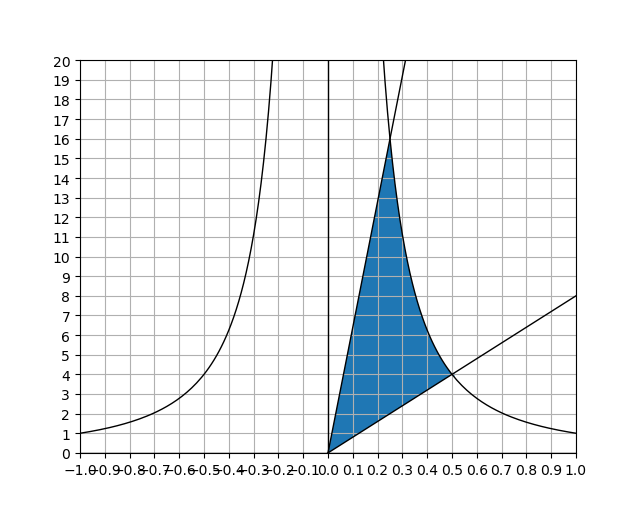
\includegraphics[width=0.6\textwidth]{q5}\par\vspace{1cm}
\item %q14b
We must start by finding all intersection points.

The intersection between \(y=8x\) and \(y=\frac{1}{x^2}\) is at \(x=\frac{1}{2}\).

The intersection point between \(y=64x\) and \(y=\frac{1}{x^2}\) is \(x=\frac{1}{4}\).

Our final intersection point between \(y=8x\) and \(y=64x\) is at \(x=0\).

We can plot these and label the points as follows.

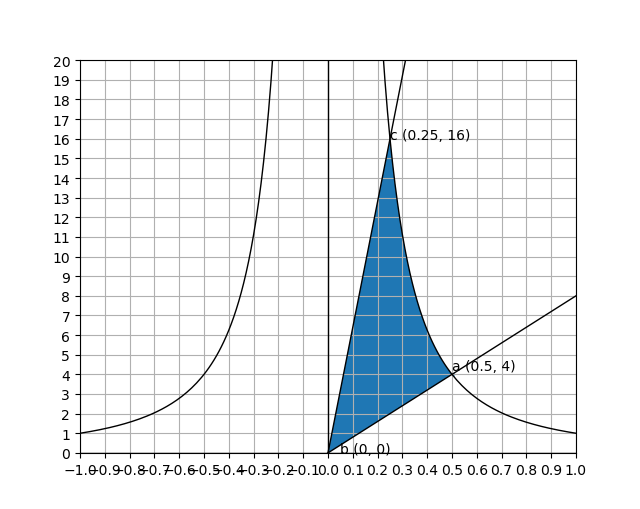
\includegraphics[width=0.6\textwidth]{q5b}\par\vspace{1cm}

We can calculate the area by separating it into a sum of two areas: 
the first area from \(x=0\) to point \(c\), or \(x=0.25\), and the second from point \(c\) onwards.

The first area between \(x=0\) and \(x=0.25\) is between lines \(y=64x\) and \(y=8x\).
It can be represented by the following integral
\[\int^\frac{1}{4}_064x-8x dx\]
Solving, we have \(56\int xdx=28x^2\).
Then, we can substitute \(x=\frac{1}{4}\) for an area of 1.75.

Next, we can represent the second area as an integral and solve.
\begin{align*}
&\int^\frac{1}{2}_\frac{1}{4}\frac{1}{x^2}-8xdx\\
\end{align*}
Let's begin by evaluating the indefinite integral.
\begin{align*}
&\int\frac{1}{x^2}-8xdx\\
&=\int \frac{1}{x^2}dx-8\int xdx\\
&=-\frac{1}{x}-4x^2
\end{align*}
Next, we can substitute \(x=0.5\) and subtract \(x=0.25\).
\[\left(-\frac{1}{0.5}-4(0.5)^2\right)-\left(-\frac{1}{0.25}-4(0.25)^2\right)=1.25\]

Adding the two areas, our final area is \(1.75+1.25=\boxed{3 \text{ square units}}\)
\end{enumerate}

\item %Q15

\item %Q16
\begin{enumerate}[label=\alph*)]
\item Let's define a function for the temperature of the bar.
Since our starting temperature is 15C and the slope is \(\frac{15}{10}=\frac{3}{2}\),
our equation is \(f(x)=\frac{3}{2}x+15\).
\[\int_0^{10} \frac{3}{2}x+15dx\]
\[\frac{3x^2}{4}+15x\]
Substituting in 10, we have \(\frac{3(10)^2}{4}+15\cdot10=225\).

However, this is the total temperature of the bar. Since the bar is 10 meters long, we must divide by 10,
and our average temperature is \(\boxed{22.5C}\)

\item We can again use our function \(f(x)=\frac{3}{2}x+15\) to find the \(x\) value where \(y=22.5\).
\[22.5=\frac{3}{2}x+15\]
\[7.5\frac{3}{2}x\]

Therefore, the average temperature of \(22.5C\) is located at \(5m\), or the center of the bar.
\end{enumerate}
\end{enumerate}
\end{document}